\subsection{Prügl}
Prügl er et spil for den tørstige hænger. I Prügl skiftes spillerne til at trække et kort fra en fordeling af kort, og derefter enten beholde eller give kortet til en anden spiller.

Traditionsmæssigt startes Prügl ved at man samler et sæt kort som alle spillere kan blive enige om er ækvivalent til et normalt kortdæk. Herefter findes en drikkevare som alle spillere higer efter. Den fundne drikkevare stilles på en overflade af passende størrelse, og kortene lægges omkring drikkevaren med forsiden nedad. Denne konstelleration af kort kaldes for en kølle\footnote{Køllen er oftest en mellemting mellem kølleformet og cirkulær, det ses dog tit at den antager andre former, såsom et hjerte, en trekant, en sol, eller en løsbunke. Formen på køllen afhænger ofte af hvor mange spil Prügl der er blevet spillet inden den aktuelle kølle.}. Et eksempel på en kølle kan ses på følgende illustration.

\begin{center}
    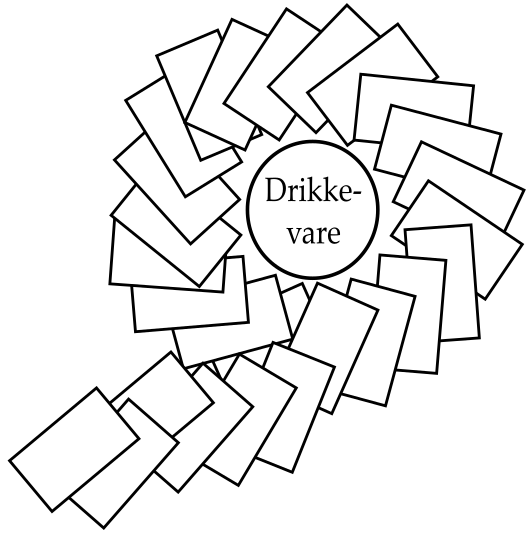
\includegraphics[width=0.75\textwidth]{../img/prugl.png}
\end{center}

Når køllen er lagt finder spilleren ud af hvem der starter: Det er selvfølgelig en ære at starte, og Prügl er et spil for folk med gode manerer, så man melder aldrig sig selv til at være den der starter.

Når den første spiller er fundet, trækker denne et vilkårligt kort fra køllen. Alt efter hvilket kort der blev trukket sker der en af følgende ting:

\begin{itemize}
    \item Sorte kort tilhører personen der har trukket dem, og lægges derfor direkte ned i egen hånd.
    \item Røde kort kan gives til en vilkårlig spiller, og man er selvgølgelig gavmild så man giver så vidt muligt røde kort til andre spillere, også selvom man selv kunne bruge kortet.
    \item Jokere er præcis det man mangler og man tager derfor selv kortet på hånden.
    \item Ruder dame og spar knægt er Ruder Helge og Spar Mogens\footnote{Eksistensgrundlaget for disse navne er åbenlyst og der vil derfor ikke blive brugt unødigt skribentarbejde på at forklare dette yderligere.}. Disse tilhøre også personen der har trukket dem, men bliver ikke taget på hånden, derimod bliver disse lagt til skue for alle spillere tæt på drikkevaren i midten af køllen.
\end{itemize}

Når den første spiller har trukket et kort går turen videre til den næste spiller i positiv omløbsretning.

For at vinde i Prügl skal summen af ens hånd være lig 25 eller ens hånd skal bestå af 5 eller flere kort. Værdien af ens hånd kan ikke overskride 25, så hvis man trækker et sort kort der ville få ens hånd til at overskride denne værdi bliver kortet desværre kasseret. Ligeledes, hvis man trækker et rødt kort og ingen spillere (ikke engang en selv) kan tage kortet uden at gå over 25 bliver det røde kort kasseret.

Jokere er altid lige det man mangler op til 25 og hvis man trækker en joker har man derfor vundet. Tillykke med det.

Spar Mogens og Ruder Helge, er så fantastisk enestående kort at hvis man trækker dem så vinder man også med det samme, 

Formålet med Prügl er at få lov til at drikke drikkevaren der står i køllen. Alle spiller er med i spillet da de alle tørster, så man vil selvfølgelig gerne vinde denne omstridte drikkevare, og skulle det hænde at man vinder modtages drikkevaren selvfølgelig med are og glæde, og i ens tørst drikkes den efter bedste evne i én enkelt slurk. De andre spillere klapper selvfølgelig for at fejre denne singulære bedrift.

Det er en uskik at køllen står tom, så alle spillere\footnote{Der ikke er optaget af andet, såsom at nyde en vinderdrikkevare.} fremskaffer i fællesskab en ny passende drikkevare som kan stå i midten af køllen

Efter vinderen har nydt sin vinderdrikkevare i et anstændigt tempo, tager denne person sin hånd, og lægger kortene til siden. Hvis vinderen skulle være i den lykkelige situation at have vundet på grund af at de har trukket Ruder Helge eller Spar Mogens, skal de dog ikke lægge deres hånd til siden, da disse korts iboende vinderegenskaber er uafhængige af kortene i en givet spillers hånd\footnote{I modsætning til en joker som jo bare er lige det man mangler på hånden for at få 25.}

Har en spiller skulle lægge deres hånd til siden så har de igen en tom hånd og kan derfor oplagt modtage nye kort. Hvis de derimod har lagt Ruder Helge eller Spar Mogens til skue, er deres hånd ufuldstændig og de kan derfor fortsætte med at tage kort på hånden. Begge tilfælde er en glædelige overraskelse da spilleren jo er utrolig tørstig og den netop nyligt fremskaffede drikkevare kan være svaret på noget af denne tørst.

Skulle uheldet være ude og køllen blive tømt for kort, så fortvivl ej; Den vakse spiller vil hurtigt opdage at der er opstået en bunke kort i nærheden af den forsvundne kølle som oplagt kan blandes og lægges omkring drikkevaren for at skabe en ny kølle, der kan bruges til at spille videre.

Således fortsætter et spil Prügl, og ens stærkt voksende tørst vil blive holdt i skak af ens medspilleres gavmildhed.
